\section{Problema}
\label{sec:problem}

Esta seção descreve o problema a solucionar e a formulação usada nas diferentes soluções.

\subsection{Descrição}
\label{subsec:description}

O jogo Tetris é uma quebra-cabeça eletrônico que consiste em empilhar peças (tetraminós) que "descem" na tela de forma a "limpar" o maior número linhas horizontais. Quando uma linha se completa, ela se desintegra, as camadas superiores descem, e o jogador ganha pontos. A partida se encerra quando a pilha de peças chega ao topo da tela e o jogador não consegue mais limpar linhas.

\begin{figure}[H]
	\centering
	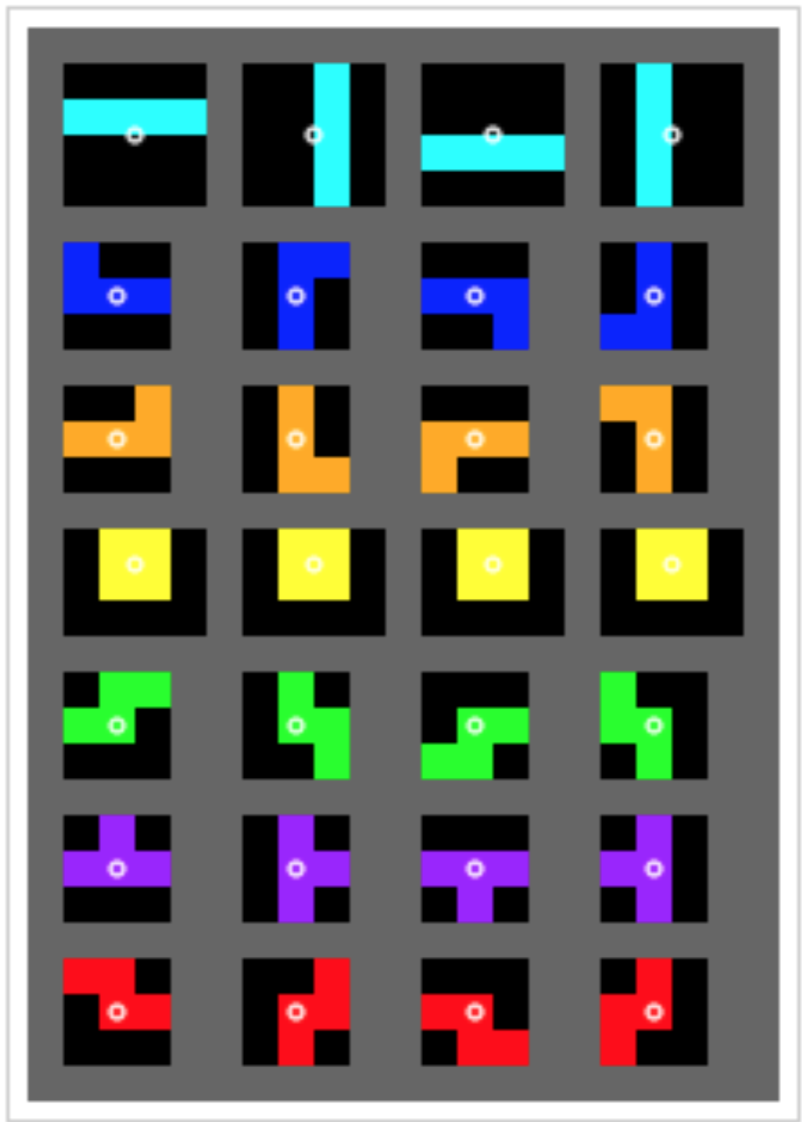
\includegraphics[height=6cm]{images/pieces}
	\caption{Os 7 tetraminós, respectivamente I, J, L, O, S, T, Z e suas possíveis rotações}
	\label{fig:tetraminos}
\end{figure}

Existem muitas variações do jogo Tetris, mas para este exercício serão adotadas as seguintes regras:

\begin{enumerate}
	\item O tabuleiro é um retângulo de 10 células de largura por 22 células de altura, isto é, 10 colunas e 22 linhas
	\item Todos os tetraminós começam no meio do tabuleiro nas linhas do topo
	\item Existem 7 tipos de tetraminós I, J, L, O, S, T, Z
	\item As ações disponíveis ao jogador são \textit{mover para esquerda} (left), \textit{mover para direita} (right) e \textit{mover para baixo} (down), que têm por efeito alterar a posição da peça em jogo nas linhas e colunas na direção desejada, \textit{despencar} (drop), que move a peça até para baixo o máximo possível, e \textit{rotacionar} (rotate), que rotaciona a peça no sentido horário
	\item Uma ação é válida em uma determinada configuração do jogo, se na configuração resultante não existe sobreposição entre a peça e as células ocupadas do tabuleiro
	\item O tempo é discreto e a cada certo número de passos (timesteps) a peça atual se desloca para baixo uma unidade automaticamente, mesmo sem ação do jogador
	\item As peças são geradas de forma aleatório e o jogador só possui conhecimento da peça atual
\end{enumerate}

A abordagem usada neste exercício ataca o problema em duas etapas: (i) formulação de meta e (ii) busca de solução. Onde (i) consiste em encontrar a melhor posição para colocar a peça atual e (ii) procura encontrar uma sequência de ações que levem a peça atual à posição meta. Só a segunda etapa vai ser explicada em detalhe para este exercício.

\subsection{Formulação do problema}
\label{subsec:formulation}

O jogo Tetris pode ser formulado da seguinte forma:

\begin{itemize}
	\item Estado: $<t , b , s>$ onde $t$ é o tetraminó ou peça atual (linha $x$, coluna $y$ e rotação), $b$ é uma matriz binaria que representa as células ocupadas do tabuleiro e $s$ é o timestep nesse instante (número de ações que o jogador ainda pode tomar antes que a peça caia automaticamente)
	\item Ações: \textit{drop, noop, left, right, down, rotate} descritas em~\ref{subsec:description}
	\item Estado inicial: a peça atual + tabuleiro vazio + timestep
	\item Estado final: tabuleiro com a peça atual na posição meta da primeira etapa
\end{itemize}

A formulação anterior será usada para desenvolver a segunda etapa do problema descrita em~\ref{subsec:description} com diferentes algoritmos de busca.